\chapter{Utilisation}
\label{sec:utilisation}

\section{Déroulement global}

Le déroulement de l'utilisation de la station de gravure laser intelligente se fait en plusieurs étapes. L'utilisateur doit d'abord dessiner le motif à graver sur l'écran tactile, puis donner la pièce au robot. Le robot prend la pièce, effectue une vérification de la prise avec la caméra et replace la pièce afin que celle-ci soit toujours dans la même position. Ensuite, le robot se positionne sous la graveuse et commence le processus de gravure. Enfin, le robot termine la gravure et remet la pièce à l'utilisateur.

\begin{figure}[H]
    \centering
    \begin{tikzpicture}[node distance=2.8cm, every node/.style={draw, align=center, rounded corners=5pt, minimum width=2.8cm, minimum height=1.1cm, font=\small}]
        \node (dessin) {Dessin sur écran tactile};
        \node (attente) [below of=dessin] {Attente de pièce};
        \node (prise) [below of=attente] {Prise de la pièce};
        \node (posi) [below of=prise] {Positionnement sous caméra};
        \node (verif) [below of=posi] {Vérification prise};
        \node (repo) [below of=verif] {Repositionnement};
        \node (placement) [below of=repo] {Placement sous la graveuse};
        \node (gravure) [below of=placement] {Gravure};
        \node (remise) [below of=gravure] {Remise à l'utilisateur};

        % Flèches principales
        \draw[->] (dessin) -- (attente);
        \draw[->] (attente) -- (prise);
        \draw[->] (prise) -- (posi);
        \draw[->] (posi) -- (verif);
        \draw[->] (verif) -- (repo);
        \draw[->] (repo) -- (placement);
        \draw[->] (placement) -- (gravure);
        \draw[->] (gravure) -- (remise);

        % Boucle retour
        \draw[->, thick] (remise.east) .. controls +(4,0) and +(4,0) .. (attente.east);
        \draw[->, dashed] (verif.west) .. controls +(-4,0) and +(-4,0) .. node[left]{Échec prise} (attente.west);
    \end{tikzpicture}
    \caption{Déroulement global de l'utilisation de la station de gravure laser intelligente}
    \label{fig:etat_utilisation}
\end{figure}

\section{Ecran tactile}

L'écran tactile est l'interface principale entre le robot et l'utilisateur. Il permet de dessiner les motifs à graver et de les envoyer.

\subsection{Démarrage de l'écran tactile}

Lors de la mise sous tension de la maquette, l'écran tactile démarre automatiquement. Cependant, il est nécessaire de lancer manuellement l'application de dessin. Pour se faire, il suffit de cliquer sur l'icône correspondant sur l'écran d'accueil. L'application se lance alors et l'utilisateur peut commencer à dessiner.

Grace à l'interface graphique développée pour l'écran tactile, l'utilisateur peut dessiner librement ce qu'il souhaite graver. A l'aide de formes prédifinies et le mode à main levée, il est possible de créer des formes et dessins variés. L'interface est claire et intuitive, permettant à l'utilisateur d'utiliser l'écran sans explications préalables.

\subsection{Interface graphique}

L'interface graphique est présentée comme suit :
\begin{figure}[H]
    \centering
    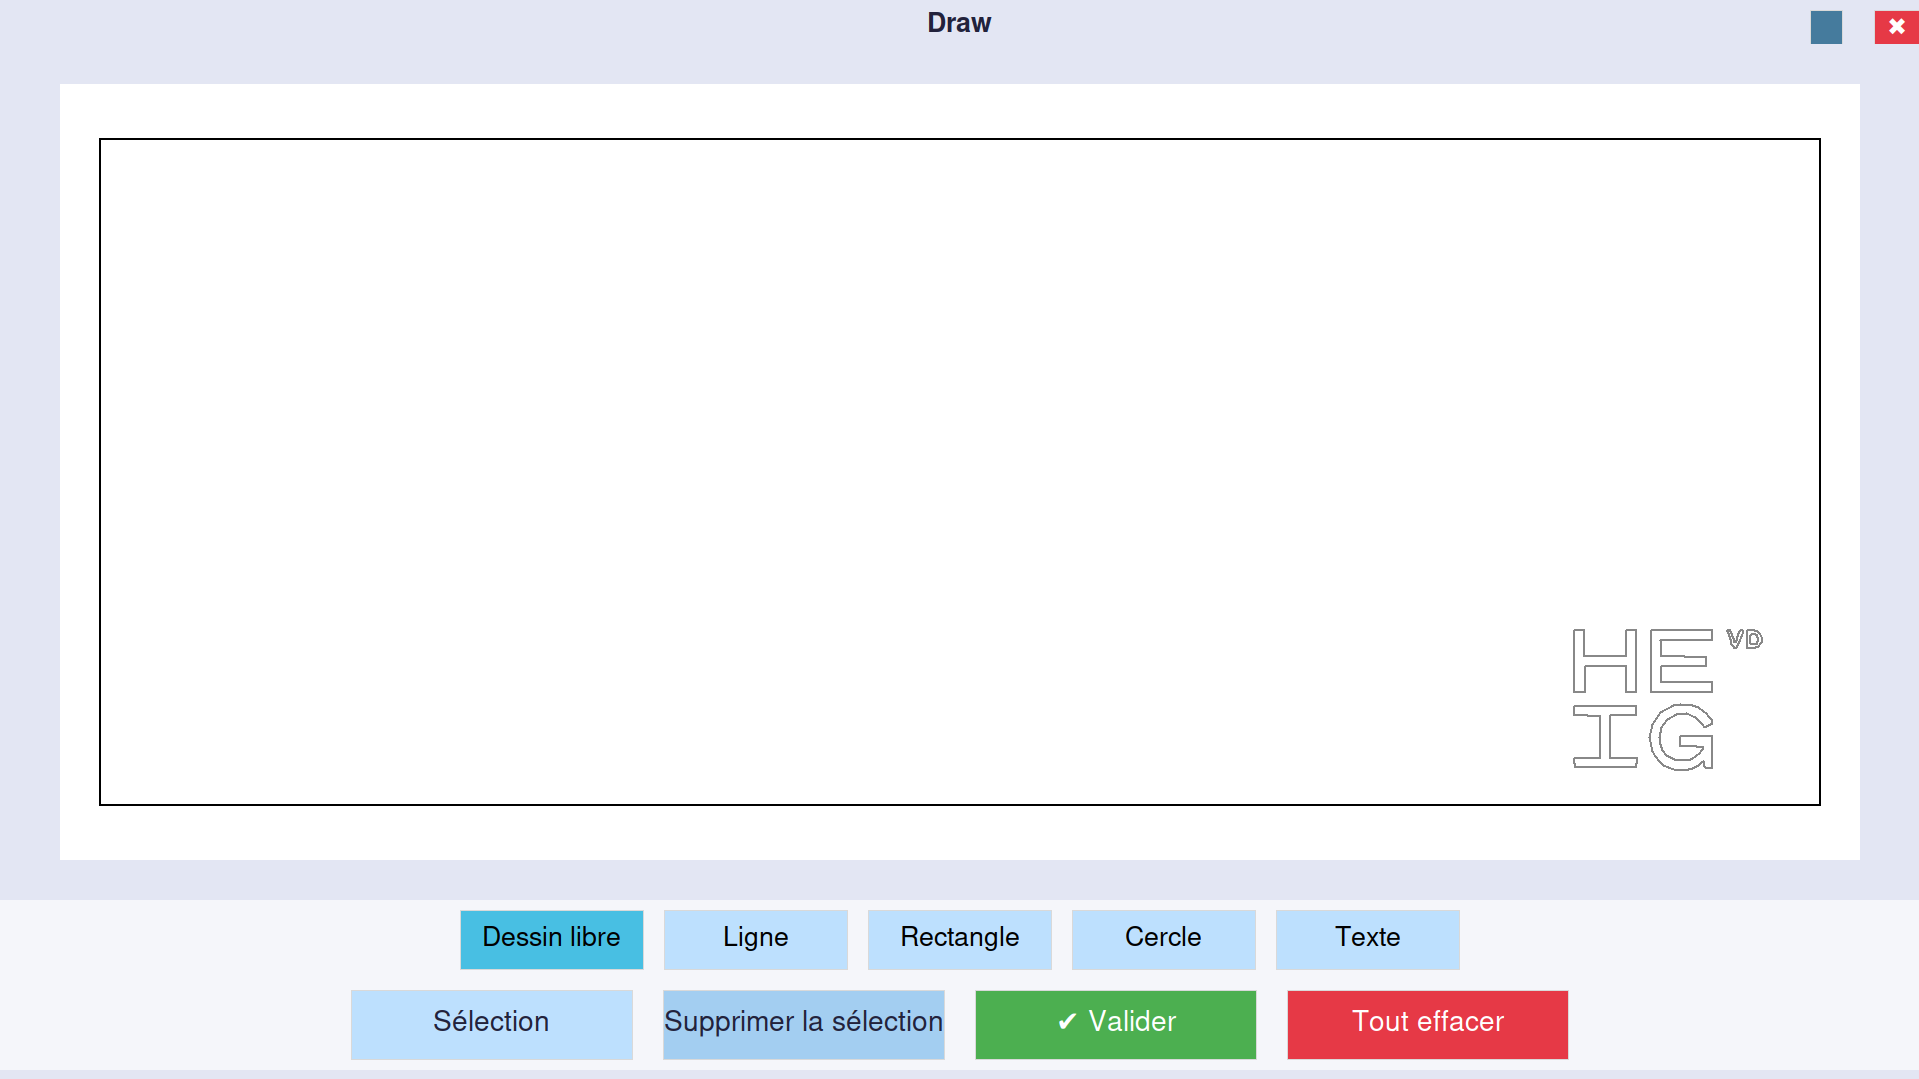
\includegraphics[width=0.8\textwidth]{assets/figures/Draw_app.png}
    \caption{Interface graphique de l'écran tactile}
    \label{fig:interface_graphique}
\end{figure}

Les codes couleurs utilisés permettent de rapidement identifier les actions possibles.

Le logo de la HEIG-VD est affiché de base sur l'application car il est gravé par défaut sur la plaque. Il n'est pas possible de supprimer le logo sans devoir modifier le code source de l'application. Cependant, il est possible de le remplacer par un autre logo en modifiant le fichier image utilisé dans le code source.


\section{AICA Studio}
Pour démarrer entièrement la maquette, il est nécessaire de démarrer le programme principal dans AICA Studio. Pour se faire, il suffit simplement de démarrer le logiciel conformément à la procédure standart linux, cliquer sur l'application voulue et appuyer sur "start". Après cela, l'application tournera en boucle tant que le bouton "Stop" n'est pas pressé.

\section{Prise de la pièce}

Après avoir dessiné et validé le dessin, l'utilisateur peut donner la pièce au robot. Le robot est constamment en attente d'une pièce à prendre. C'est à dire que dès qu'une pièce est détectée dans le zone de prise, le robot se déplacera pour la prendre. Il est important de noter que le programme ne vérifie pas si un nouveau dessin a été fait avant de prendre la pièce. Il est donc possible de donner une pièce au robot sans avoir dessiné au préalable. Le robot utilisera donc le dernier dessin envoyé au programme.

\subsection{Prérequis}

Le programme est conçu pour prendre la pièce uniquement dans des conditions spécifiques afin d'assurer la sécurité et la fiabilité du processus. Ces conditions sont les suivantes :
\begin{itemize}
    \item La pièce doit être placée dans la zone de prise du robot.
    \item La pièce doit être détectée par le bloc de détection, selon plusieurs critères :
          \begin{itemize}
              \item La couleur de la pièce doit correspondre à celle définie dans le bloc fonctionnel de la caméra.
              \item La taille de la pièce doit être ni trop grande ni trop petite.
              \item La pièce doit correspondre au modèle 3D à un certain pourcentage.
          \end{itemize}
\end{itemize}

Tous ces paramètres sont vérifiés par le programme avant de prendre la pièce. Si l'une de ces conditions n'est pas remplie, le robot ne prendra pas la pièce et restera en position d'attente. Dans le cas ou le robot est sur le point de prendre la pièce et que celle-ci n'est pas détectée, le robot retournera en position d'attente.

\subsection{Inconvénients}

A cause de la complexité de la détection de la pièces, des règles de détection et de la couleur de la pièce, il est possible que le programme ne détecte pas correctement la pièce à cause de la couleur de peau de l'utilisateur. En effet, comme expliqué précédement, une partie du traitement de l'image utilise la couleur de la pièce pour isoler le nuage de points correspondant à la pièce. Si la couleur de peau de l'utilisateur est proche de celle de la pièce, le programme risque de ne pas détecter correctement la pièce. Il est donc parfois obligatoire de porter des gants de couleur différente de celle de la pièce pour que le robot puisse prendre la pièce correctement.

\begin{figure}[H]
    \centering
    \begin{subfigure}{0.48\textwidth}
        \centering
        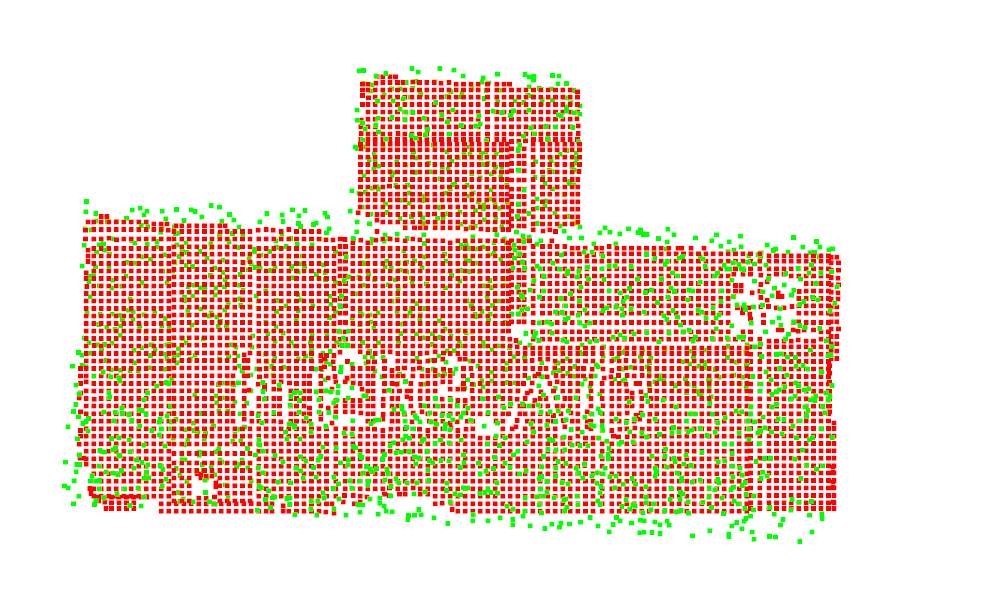
\includegraphics[width=0.95\linewidth]{assets/figures/bonne_detec.png}
        \caption{Bonne détection de la pièce}
        \label{fig:bonne_detection_piece}
    \end{subfigure}
    \hfill
    \begin{subfigure}{0.48\textwidth}
        \centering
        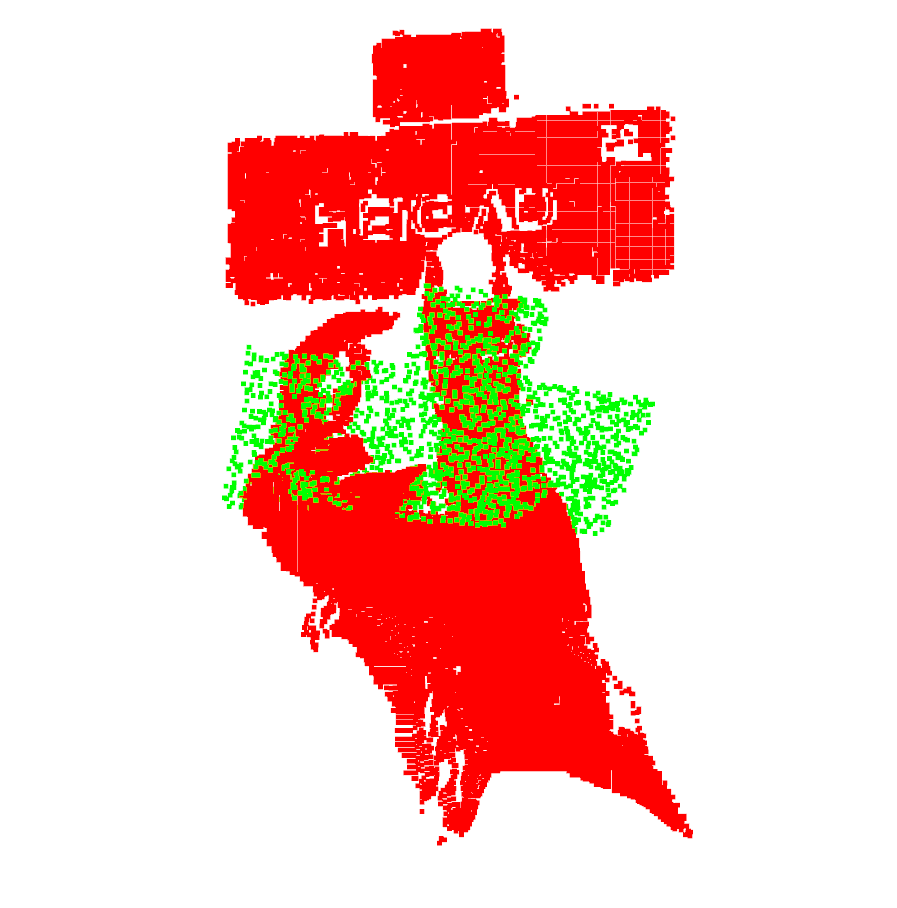
\includegraphics[width=0.95\linewidth]{assets/figures/mauvaise_detec.png}
        \caption{Mauvaise détection de la pièce}
        \label{fig:mauvaise_detection_piece}
    \end{subfigure}
    \caption{Exemples de détection bonne et mauvaise de la pièce}
    \label{fig:comparaison_detection_piece}
\end{figure}

\subsection{Préhension}

Lorsque la pièce est tendue au robot par l'utilisateur dans les bonnes conditions, le robot se déplace alors vers la position de la pièce et se rapproche le plus possible. Quand le programme détermine que la pièce est suffisamment proche de la pince à l'aide d'un bloc de collision, le robot ferme la pince pour prendre la pièce. Il est important de noter que le robot ne vérifie pas si la pièce est bien prise avant de se déplacer vers la zone de gravure. Cela demande trop de temps et de complexité au programme. Cependant, le robot effectue tout de même un replacement de la pièce après la prise pour s'assurer que la pièce est bien placée pour la gravure.

\begin{figure}[H]
    \centering
    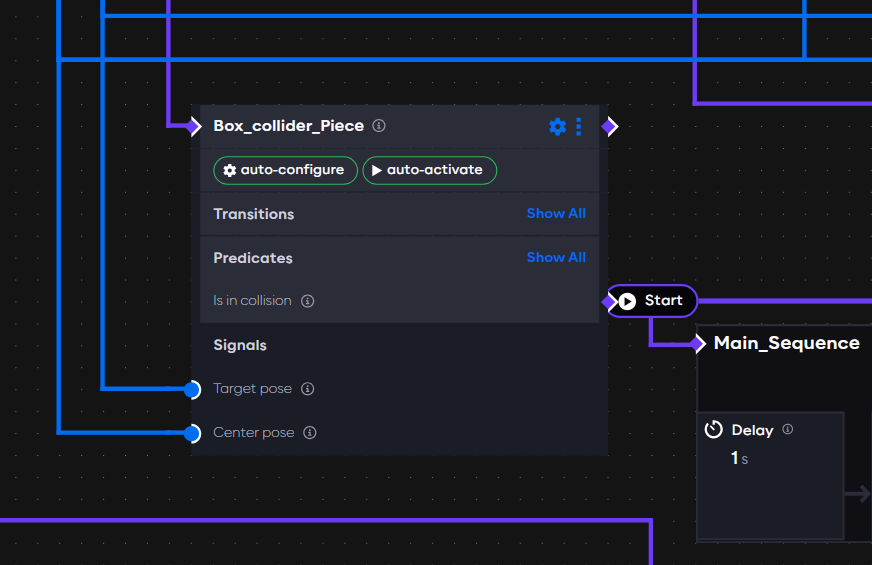
\includegraphics[width=0.8\textwidth]{assets/figures/AICA_box_prise.png}
    \caption{Bloc fonctionnel de collision pour la fermeture de la pince}
    \label{fig:prise_piece}
\end{figure}

\section{Gravure de la pièce}

La gravure de la pièce se fait automatiquement après la prise de celle-ci. Le robot se déplace alors vers la zone de gravure et commence à graver le dessin précédemment dessiné par l'utilisateur.

